\documentclass[11pt]{article}

\usepackage{sectsty}
\usepackage{graphicx}
\usepackage{enumitem}
\usepackage{listings}
\usepackage{xcolor}
\usepackage{graphicx}
\usepackage{fancyhdr}
\usepackage{epigraph} 

\definecolor{codegreen}{rgb}{0,0.6,0}
\definecolor{codegray}{rgb}{0.5,0.5,0.5}
\definecolor{codepurple}{rgb}{0.58,0,0.82}
\definecolor{backcolour}{rgb}{0.95,0.95,0.92}

\lstdefinestyle{mystyle}{
    backgroundcolor=\color{backcolour},   
    commentstyle=\color{codegreen},
    keywordstyle=\color{magenta},
    numberstyle=\tiny\color{codegray},
    stringstyle=\color{codepurple},
    basicstyle=\ttfamily\footnotesize,
    breakatwhitespace=false,         
    breaklines=true,                 
    captionpos=b,                    
    keepspaces=true,                 
    numbers=left,                    
    numbersep=5pt,                  
    showspaces=false,                
    showstringspaces=false,
    showtabs=false,                  
    tabsize=2
}

\lstset{style=mystyle}


% Margins
\topmargin=-0.45in
\evensidemargin=0in
\oddsidemargin=0in
\textwidth=6.5in
\textheight=9.0in
\headsep=0.25in

\title{ Web Technology Solution\\2020 Fall}

\author{ Sanjaya (Bir Bikram) Shrestha }
\date{\today}



\begin{document}
\maketitle	
\pagestyle{fancy}
\fancyhead[RO,LE]{\textbf{WT Solution 2020 Fall}}
\fancyfoot[RO,RE]{By: Sanjaya (Bir Bikram) Shrestha}

\tableofcontents
\pagebreak

% Optional TOC
% \tableofcontents
% \pagebreak

%--Paper--
\noindent\rule{\linewidth}{0.4pt}
\section{(Q No.1 A) What is Web Standard? Explain different types of web standards available in web technology with example. }
\subparagraph{}
Web standards refer to a set of guidelines, specifications, and best practices developed by the World Wide Web Consortium (W3C) and other organizations to ensure the interoperability, accessibility, and usability of web content across different devices, platforms, and browsers.

There are several types of web standards available in web technology, including:

\begin{enumerate}
    \item HTML Standards: HTML is the markup language used to structure and present web content. The latest version of HTML is HTML5, which includes new features such as multimedia support, form controls, and semantic tags. HTML standards ensure that web pages are correctly formatted and easily readable by both humans and machines.

    \item CSS Standards: Cascading Style Sheets (CSS) are used to control the visual presentation of web content. CSS standards ensure that web pages are visually consistent across different devices, platforms, and browsers. For example, CSS3 includes new features such as responsive design, animations, and transitions.
    
    \item JavaScript Standards: JavaScript is a programming language used to add interactivity and dynamic behavior to web pages. JavaScript standards ensure that web pages are responsive and interactive, and that they work correctly across different devices and platforms. For example, the ECMAScript 6 standard introduced new features such as arrow functions, classes, and modules.
    
    \item Accessibility Standards: Accessibility standards ensure that web content is accessible to people with disabilities, such as visual, auditory, and motor impairments. The Web Content Accessibility Guidelines (WCAG) are a set of guidelines developed by the W3C to ensure that web content is perceivable, operable, understandable, and robust.
    
    \item Security Standards: Security standards ensure that web content is secure and protected against unauthorized access, data breaches, and other security threats. For example, the HTTPS protocol encrypts web traffic to ensure that sensitive information, such as passwords and credit card numbers, is transmitted securely.
\end{enumerate}


\noindent\rule{\linewidth}{0.4pt}
\section{(Q No.1B) Define DNS? Explain the uses of following protocols in Web Technology with example.}
\begin{enumerate}
    \item HTTP
    \item FTP
    \item POP
\end{enumerate}
\subparagraph{}
DNS stands for Domain Name System. It is a hierarchical decentralized naming system that translates human-readable domain names, such as www.example.com, into the numerical IP addresses that computers use to identify each other on the internet.

DNS servers maintain a distributed database of domain names and their corresponding IP addresses, which allows devices to easily locate and communicate with each other over the internet. When a user types a domain name into their web browser, the browser sends a request to a DNS server to resolve the domain name into an IP address. The DNS server responds with the IP address, allowing the browser to establish a connection with the desired website.
\begin{enumerate}
    \item \textbf{HTTP}
    HTTP stands for Hypertext Transfer Protocol, and it is the protocol that underlies the World Wide Web. It is a protocol that defines how clients and servers communicate over the internet.

    HTTP works by establishing a connection between a client, such as a web browser, and a server, which hosts the content the client is requesting. The client sends an HTTP request to the server, specifying the URL of the resource it wants to access, such as a web page or an image. The server then responds with an HTTP response, which contains the requested resource or an error message if the request cannot be fulfilled.

    HTTP requests and responses are composed of headers and, optionally, a message body. The headers contain information about the request or response, such as the type of content being sent, the encoding used, and any cookies or authentication tokens required. The message body contains the actual content being sent, such as HTML, CSS, JavaScript, images, or video.

    \item \textbf{FTP} stands for File Transfer Protocol, and it is a protocol used to transfer files between computers over the internet.

    FTP works by establishing a connection between a client, which is usually a computer, and a server, which hosts the files the client wants to access or transfer. The client sends an FTP request to the server, specifying the file(s) it wants to access or transfer. The server then responds with an FTP response, which contains the requested file(s) or an error message if the request cannot be fulfilled.
    
    FTP requests and responses are composed of commands and replies, which are sent over a control connection established between the client and the server. The commands instruct the server to perform certain actions, such as listing the files in a directory, downloading a file, or uploading a file. The replies contain information about the status of the command, such as whether it was successful or not.
    \item \textbf{POP} stands for Post Office Protocol, and it is a protocol used to retrieve email messages from a mail server.

    POP works by establishing a connection between an email client, such as Microsoft Outlook or Apple Mail, and a mail server, which hosts the user's email messages. The client sends a POP request to the server, specifying the user's credentials and the messages they want to access. The server then responds with a POP response, which contains the requested messages or an error message if the request cannot be fulfilled.
    
    POP requests and responses are composed of commands and replies, which are sent over a TCP connection established between the client and the server. The commands instruct the server to perform certain actions, such as listing the messages in a mailbox, downloading a message, or deleting a message. The replies contain information about the status of the command, such as whether it was successful or not.
\end{enumerate}

\noindent\rule{\linewidth}{0.4pt}
\section{(Q No.2A) Write HTMl tags for the following form}
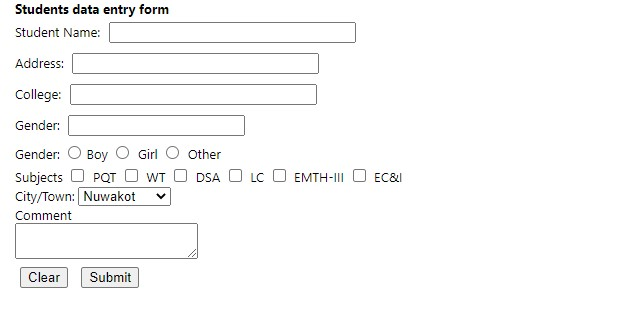
\includegraphics[width=0.75\textwidth]{resources/qno2a.jpg}
Here is the source code of the given form:
\lstinputlisting[language=html, caption={Html Form}]{resources/qno2a.html}

\noindent\rule{\linewidth}{0.4pt}
\section{(Q No.2B) What are the two required attribute of $<$img$>$ tag in HTML? Describe different types of multimedia format used in HTML with example.}
\subparagraph{}
The two required attributes of the $<$img$>$ tag in HTML are src and alt.

The src attribute specifies the URL of the image file that should be displayed. \\
The alt attribute provides alternative text that should be displayed if the image cannot be loaded, or for users who are visually impaired and using assistive technology to access the content. It should describe the content or purpose of the image. \\
For example:
\begin{lstlisting}
    <img src="https://example.com/images/cat.jpg" alt="A cute cat">
\end{lstlisting}

HTML supports a different types of multimedia formats, here are some examples:
\begin{enumerate}
    \item \textbf{Audio:} HTML supports the $<$audio$>$ tag for playing audio files. Supported formats include MP3, WAV, and OGG.
    \begin{lstlisting}
        <audio src="https://example.com/audio/song.mp3" controls></audio>
    \end{lstlisting}
    \item \textbf{Video:} HTML supports the $<$video$>$ tag for displaying videos. Supported formats include MP4, WebM, and OGG.
    \begin{lstlisting}
        <video src="https://example.com/videos/video.mp4" controls></video>
    \end{lstlisting}
    \item \textbf{Animated images:} HTML supports the $<$canvas$>$ tag for displaying animated images created using JavaScript or other scripting languages.
    \begin{lstlisting}
        <canvas id="myCanvas"></canvas>
    \end{lstlisting} 
\end{enumerate}


\noindent\rule{\linewidth}{0.4pt}
\section{(Q No.3A) What is the purpose of CSS? List out Different Types of CSS Selectors. Explain box model in CSS with suitable figure. }
\subparagraph{}
CSS stands for Cascading Style Sheets. Its main purpose is to separate the presentation of a web page from its content, allowing developers to control the layout, typography, colors, and other visual aspects of a website or web application.
Here are some common types of CSS selectors:

\begin{enumerate}
    \item \textbf{Element selector:} Targets all instances of a specific HTML element. For example, to style all paragraphs on a page:
    \begin{lstlisting}
        p {
            color: red;
        }
    \end{lstlisting} 
    \item \textbf{Class selector:} Targets all instances of an HTML element with a specific class. For example, to style all elements with the class "highlight":
    \begin{lstlisting}
        .highlight {
            background-color: yellow;
        }
    \end{lstlisting}
    \item ID selector: Targets a single HTML element with a specific ID. For example, to style an element with the ID "header":
    \begin{lstlisting}
        #header {
            font-size: 24px;
        }
    \end{lstlisting}
    \item Attribute selector: Targets HTML elements based on their attributes. For example, to style all links with a "target" attribute:
    \begin{lstlisting}
        a[target="_blank"] {
            color: blue;
        }  
    \end{lstlisting}

\end{enumerate}
The CSS box model is a container that contains multiple properties including borders, margin, padding, and the content itself. It is used to create the design and layout of web pages. It can be used as a toolkit for customizing the layout of different elements. The web browser renders every element as a rectangular box according to the CSS box model. Box-Model has multiple properties in CSS. \\

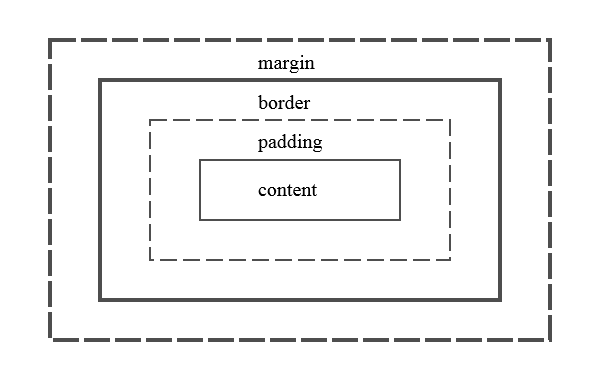
\includegraphics[width=0.75\textwidth]{resources/cssbox.png}

\noindent\rule{\linewidth}{0.4pt}
\section{(Q No.3B) Define DOM. Differentiate betweeen DOM 0 and DOM 2 event models in JavaScript with suitable examples.} 
DOM (Document Object Model) is a hierarchical tree-like structure that represents the elements, attributes, and text content of an HTML or XML document. Each node in the tree represents a different part of the document, such as the document itself, an HTML element, or a piece of text.

DOM 0 and DOM 2 are two different event models in JavaScript that are used to handle events in web applications. Here are the main differences between these two models, along with examples:
\begin{itemize}
    
    \item DOM 0 Event Model:

        This is the original event model in JavaScript.
        In this model, event handlers are attached directly to HTML elements using inline event handlers or the element.onclick property.
        Example:
        \begin{lstlisting}
            <button onclick="alert('Hello world!')">Click me</button>
        \end{lstlisting}

        \begin{lstlisting}[language=html]
            const button = document.querySelector('button');
            button.onclick = function() {
            alert('Hello world!');
            };
        \end{lstlisting}
    \item DOM 2 Event Model:

        This is a newer event model that was introduced in JavaScript.
        In this model, event handlers are attached to HTML elements using the addEventListener() method.
        This method takes two arguments: the name of the event to listen for, and a function that will be called when the event occurs.
        Multiple event listeners can be added to the same element for the same event.
        \begin{lstlisting}
            <button id="myButton">Click me</button>
        \end{lstlisting}

        \begin{lstlisting}
            const button = document.querySelector('#myButton');
            button.addEventListener('click', function() {
            alert('Hello world!');
            });
        \end{lstlisting}



\end{itemize}


\noindent\rule{\linewidth}{0.4pt}
\section{(Q No.4A) What is the difference betweeen == and === in JavaScript? Write down the different data types in JavaScript with example.} 
\subparagraph{}
In JavaScript, == and === are both comparison operators used to compare values. \\
The key differences are:\\
The == operator is the loose or abstract equality operator. It compares values for equality after converting both operands to a common type. If the two values being compared are of different types, JavaScript will try to convert one or both values to a common type before comparing them. For example:
\begin{lstlisting}
    1 == "1"; // true
    null == undefined; // true
    true == 1; // true
\end{lstlisting}
In the examples above, the == operator compares values after converting them to a common type. In the first example, the string "1" is converted to the number 1 before comparison. In the second example, both null and undefined are considered equal. In the third example, the boolean value true is converted to the number 1 before comparison.

On the other hand, the === operator is the strict equality operator. It compares values for equality without type conversion. If the two values being compared are of different types, the result is always false. For example:
\begin{lstlisting}
    1 === "1"; // false
    null === undefined; // false
    true === 1; // false
\end{lstlisting}
In the examples above, the === operator compares values without converting them to a common type. In all three examples, the result is false because the types of the values being compared are different.

The different data types are:
\begin{enumerate}
    \item \textbf{Numbers:} numeric values, including integers and floating-point numbers. Example: 42, 3.14.

    \item \textbf{Strings:} textual data enclosed in quotes. Example: "Hello, World!", 'JavaScript is awesome'.
    
    \item \textbf{Booleans:} logical values that can be either true or false. Example: true, false.
    
    \item \textbf{Null:} a special value indicating the absence of any object value. Example: null.
    
    \item \textbf{Undefined:} a special value indicating that a variable has not been assigned a value. Example: undefined.
    
    \item \textbf{Objects:} complex data structures made up of key-value pairs, arrays, and functions. Example: { name: "John", age: 30 }.
    
    \item \textbf{Arrays:} ordered lists of values, which can be of any data type. Example: [1, 2, 3, 4].
    
    \item \textbf{Functions:} blocks of code that can be called and executed when needed. Example: function add(a, b) { return a + b; }.
\end{enumerate}


\noindent\rule{\linewidth}{0.4pt}
\section{(Q No.4B) How can we locate the mouse cursor and react to the mouse clicks in JavaScript? Explain with example. } 
\subparagraph{}
In JavaScript, you can use the MouseEvent object to locate the position of the mouse cursor and react to mouse clicks. Here's an example:
\begin{lstlisting}
    // Add an event listener for mouse clicks on the document
    document.addEventListener("click", function(event) {
    // Get the X and Y coordinates of the mouse cursor
    var x = event.clientX;
    var y = event.clientY;
    
    // Log the coordinates to the console
    console.log("Mouse clicked at (" + x + ", " + y + ")");
    });
\end{lstlisting}
In the code above, we've added an event listener to the document object for the "click" event. Whenever the user clicks anywhere on the document, the function passed to the addEventListener method will be executed. Inside this function, we're using the clientX and clientY properties of the MouseEvent object to get the X and Y coordinates of the mouse cursor at the time of the click. We then log these coordinates to the console using console.log.

We can also use the mousedown, mouseup, and mousemove events to react to mouse actions other than clicks. The mousedown event is fired when a mouse button is pressed down, mouseup is fired when a mouse button is released, and mousemove is fired when the mouse pointer is moved over an element.


\noindent\rule{\linewidth}{0.4pt}
\section{(Q No.5A) Why PHP is called server side scripting language? Explain control statements in PHP with examples.} 
PHP is called a server-side scripting language because it runs on the server-side, meaning the code is executed on the web server before the resulting HTML page is sent to the client-side browser. This is different from client-side scripting languages like JavaScript, which run on the client-side browser.

Control statements in PHP are used to control the flow of execution in a PHP script. There are several types of control statements in PHP, including if/else statements, switch statements, loops, and more. Here are some examples:

\begin{itemize}
    \item \textbf{If/else statement:}
    The if/else statement is used to execute code based on a condition. If the condition is true, the code in the if block is executed, otherwise, the code in the else block is executed.
    
    \begin{lstlisting}[language=php]
        $num = 10;
        if ($num > 5) {
        echo "The number is greater than 5";
        } else {
        echo "The number is less than or equal to 5";
        }
    \end{lstlisting}

    \item \textbf{Switch statement:}
    The switch statement is used to execute different blocks of code based on different conditions.
    It contains a switch keyword which needs condition to match with the case, else it goes for default  section. "break" keyword is used on each case to exit the block.
    \begin{lstlisting}[language=php]
        $color = "red";
        switch ($color) {
        case "red":
            echo "The color is red";
            break;
        case "blue":
            echo "The color is blue";
            break;
        default:
            echo "The color is not red or blue";
            break;
        }

    \end{lstlisting}
    
    \item \textbf{Loops:}
    Loops are used to execute a block of code multiple times. in PHP we have 4 types of loop.
    \begin{itemize}
        
        \item \textbf{while -} loops through a block of code as long as the specified condition is true
        \item \textbf{do...while -} loops through a block of code once, and then repeats the loop as long as the specified condition is true
        \item \textbf{for - loops} through a block of code a specified number of times
        \item \textbf{foreach -} loops through a block of code for each element in an array
     
    \end{itemize}
    \begin{lstlisting}[language=php]
        // For loop
        for ($i = 0; $i < 10; $i++) {
        echo $i;
        }

        // While loop
        $i = 0;
        while ($i < 10) {
        echo $i;
        $i++;
        }

        // Do-while loop
        $i = 0;
        do {
        echo $i;
        $i++;
        } while ($i < 10);

        $ages = array("John" => 30, "Jane" => 25, "Bob" => 40);

        foreach ($ages as $name => $age) {
        echo $name . " is " . $age . " years old.<br>";
        }


    \end{lstlisting}

\end{itemize}


\noindent\rule{\linewidth}{0.4pt}
\section{(Q No.5B) Differentiate cookie and session. Explain with an php program.} 
\subparagraph{}

Session and cookies are two ways to store data between HTTP requests in PHP. Here are some key differences:

\begin{enumerate}
    \item \textbf{Storage Location:} Session data is stored on the server, while cookie data is stored on the client (in the browser).

    \item \textbf{Data Size:} Cookies have a maximum size limit of around 4 KB, while session data can be much larger.
    
    \item \textbf{Security:} Session data is generally considered more secure than cookies, as it is stored on the server and cannot be easily tampered with by the client.
    
    \item \textbf{Expiration:} Cookies can have an expiration date, while session data is destroyed when the user closes their browser or logs out.
    
    \item \textbf{Accessibility:} Cookies can be accessed by both the client-side scripts and server-side scripts, while session data can only be accessed by server-side scripts.
    \item Cookies can be set using the setcookie() function. This function takes several parameters including the cookie name, value, expiration time, and path.
    \begin{lstlisting}[language=php]
        setcookie('username', 'john_doe', time() + 3600, '/');
    \end{lstlisting}
    For Retrieving data from cookie we use following code:
    \begin{lstlisting}[language=php]
        // Check if the 'username' cookie is set and retrieve its value
        if (isset($_COOKIE['username'])) {
        $username = $_COOKIE['username'];
        echo "Welcome back, $username!";
        } else {
        echo "Please log in to continue.";
        }
    \end{lstlisting}
    For starting session and setting values in it we use following code:
    \begin{lstlisting}[language=php]
        // Start the session
        session_start();

        // Check if the 'username' session variable is set and retrieve its value
        if (isset($_SESSION['username'])) {
        $username = $_SESSION['username'];
        echo "Welcome back, $username!";
        } else {
        echo "Please log in to continue.";
        }

    \end{lstlisting}
\end{enumerate}



\noindent\rule{\linewidth}{0.4pt}
\section{(Q No.6A) In what ways can arrays in PHP be created? How can we access array elements? Briefly describe functions for dealing with arrays in PHP. } 
\subparagraph{}
In PHP, there are several ways to create arrays:

\begin{enumerate}
    \item Using the array() function:
    \begin{lstlisting}[language=php]
        $myArray = array("apple", "banana", "orange");
    \end{lstlisting}
    \item Using the [] shorthand syntax:
    \begin{lstlisting}[language=php]
        $myArray = ["apple", "banana", "orange"];
    \end{lstlisting}
    \item Using the range() function to create an array with a range of values:
    \begin{lstlisting}[language=php]
        $myArray = range(1, 10);
    \end{lstlisting}
    \item Using the explode() function to create an array from a string:
    \begin{lstlisting}[language=php]
        $myString = "apple,banana,orange";
    $myArray = explode(",", $myString);

    \end{lstlisting}

    Once array is created in PHP, we can access its elements using the square bracket notation for indexed array:
    \begin{lstlisting}[language=php]
        $myArray = array("apple", "banana", "orange");
        echo $myArray[0]; // Output: apple
        echo $myArray[1]; // Output: banana
        echo $myArray[2]; // Output: orange

    \end{lstlisting}
    For associative array we can index using thier string index
    \begin{lstlisting}[language=php]
        $salaries = array("mohammad" => 2000, "qadir" => 1000, "zara" => 500);
        echo "Salary of mohammad is ". $salaries['mohammad'] . "<br />";
        echo "Salary of qadir is ".  $salaries['qadir']. "<br />";
        echo "Salary of zara is ".  $salaries['zara']. "<br />"
    \end{lstlisting}
\end{enumerate}
Some built in array function in PHP are:

\begin{enumerate}
    \item count(): Returns the number of elements in an array.
    \item sort(): Sorts an array in ascending order.
    \item rsort(): Sorts an array in descending order.
    \item array\_push(): Adds one or more elements to the end of an array.
    \item array\_pop(): Removes the last element from an array.
\end{enumerate}


\noindent\rule{\linewidth}{0.4pt}
\section{(Q No.6B) Make a login form with e-mail and password. Write a program to make dynamic login using PHP and MySQL query. Your program must contain a database connection file from php to MySQL.} 
\subparagraph{}
Here is the source code for given scenario.

\lstinputlisting[language=html, caption={Login Page: index.html}]{resources/qno6.html}

\lstinputlisting[language=php, caption={Login Page: login.php}]{resources/qno6.php}


In the above code, we start the session and establish a database connection using mysqli\_connect(). We then check if the login form is submitted by checking if the \$\_POST array contains values for username and password fields. We also check if the user has checked the "remember me" checkbox, and if so, we set cookies to remember the login session for 30 days.

We then use mysqli\_real\_escape\_string() to sanitize the entered username and password, and execute a query to retrieve the user with the given credentials from the database. If the query returns a row, we create a session variable named 'username' and set it to the entered username, and then redirect the user to the homepage. If the query doesn't return any rows, we display an error message.

Finally, we close the database connection using mysqli\_close().
Here We have some basic validation in client side using JavaScript which will check for null value, password should be at least 8 character and email patter using regular expression. Once every validaion is passed then we submit form to the server, login.php. 


\noindent\rule{\linewidth}{0.4pt}
\section{(Q No.7A) Stacking element in JavaScript} 
\subparagraph{}
In JavaScript, we can stack HTML elements using the DOM (Document Object Model). The DOM is a programming interface for HTML and XML documents, which provides a way to access and manipulate the structure and content of a document.

To stack HTML elements using the DOM, we can create a parent container element and add child elements to it. The child elements will be stacked vertically or horizontally, depending on the layout style applied to the parent container.

Here is an example of stacking HTML elements vertically using the DOM:

\begin{lstlisting}[language=html]
    <div id="container"></div>

    // Get a reference to the parent container element
    var container = document.getElementById("container");

    // Create some child elements to stack
    var element1 = document.createElement("div");
    element1.innerHTML = "Element 1";

    var element2 = document.createElement("div");
    element2.innerHTML = "Element 2";

    var element3 = document.createElement("div");
    element3.innerHTML = "Element 3";

    // Add the child elements to the parent container element
    container.appendChild(element1);
    container.appendChild(element2);
    container.appendChild(element3);

\end{lstlisting}

In this example, we create a parent container element with the ID "container". We then create three child elements (divs) with some text content and add them to the parent container element using the appendChild() method. The child elements are added to the end of the container element, which results in a vertical stack.

We can also stack elements horizontally by applying a layout style to the parent container element. Here is an example:
\begin{lstlisting}[language=html]
    <div id="container" style="display: flex;"></div>

    // Get a reference to the parent container element
    var container = document.getElementById("container");

    // Create some child elements to stack
    var element1 = document.createElement("div");
    element1.innerHTML = "Element 1";

    var element2 = document.createElement("div");
    element2.innerHTML = "Element 2";

    var element3 = document.createElement("div");
    element3.innerHTML = "Element 3";

    // Add the child elements to the parent container element
    container.appendChild(element1);
    container.appendChild(element2);
    container.appendChild(element3);

\end{lstlisting}
In this example, we add a display: flex style to the parent container element using the style attribute. This applies a flexible box layout to the container element, which allows the child elements to be stacked horizontally. The child elements are still added using the appendChild() method, but they will be positioned horizontally instead of vertically.


\section{(Q No.7B) Dynamic Content in JavaScript} 
\subparagraph{}
Dynamic content in JavaScript refers to the ability to change the content of a web page at runtime, based on user interactions, data inputs, or other external factors. With dynamic content, we can create rich and interactive web interfaces that respond to user actions and provide real-time feedback.

There are many ways to add dynamic content to a web page using JavaScript. Here are some common techniques:

\begin{itemize}
    \item \textbf{DOM Manipulation:} With the Document Object Model (DOM), we can add, remove, or modify HTML elements and their attributes dynamically. We can use methods like createElement(), appendChild(), setAttribute(), and innerHTML to manipulate the DOM and update the content of a web page.

    \item \textbf{Event Handling:} By registering event listeners on HTML elements, we can trigger JavaScript functions in response to user interactions, such as clicks, keystrokes, and form submissions. We can use event handling to validate user input, perform calculations, or update the content of a web page based on user actions.
\end{itemize}
    
    \begin{lstlisting}[language=html]
        <button id="button">Click me</button>
        <div id="content"></div>

        // Get a reference to the button element
        var button = document.getElementById("button");

        // Add an event listener to the button
        button.addEventListener("click", function() {
        // Get a reference to the content element
        var content = document.getElementById("content");
        
        // Create a new element to add to the content
        var message = document.createElement("p");
        message.innerHTML = "You clicked the button!";
        
        // Add the message to the content
        content.appendChild(message);
        });

    \end{lstlisting}
we add a button element and a content element to the HTML. We then use JavaScript to add an event listener to the button that responds to clicks. When the button is clicked, we use DOM manipulation to create a new paragraph element with a message and add it to the content element. This results in dynamic content that is added to the web page based on user interactions.

\section{(Q No.7C) CRUD Operation in MySQL} 
CRUD stands for Create, Read, Update, and Delete, which are the basic operations used to manipulate data in a database. Here's an example of how to perform CRUD operations in MySQL using PHP:

\begin{enumerate}
    \item \textbf{Create:} To create a new record in the database, we use the INSERT statement in SQL. Here's an example of inserting data into a users table:

    \item \textbf{Read:} To read data from the database, we use the SELECT statement in SQL. Here's an example of selecting data from a users table:
    
    \item \textbf{Update:} To update an existing record in the database, we use the UPDATE statement in SQL. Here's an example of updating data in a users table:
    
    \item \textbf{Delete:} To delete a record from the database, we use the DELETE statement in SQL. Here's an example of deleting data from a users table:
\end{enumerate}
Here is sample example for CRUD Operation in MySql usin PHP:

\begin{lstlisting}[language=php]
    <?php
    // Connect to the database
    $host = 'localhost';
    $user = 'username';
    $password = 'password';
    $dbname = 'database_name';
    $conn = mysqli_connect($host, $user, $password, $dbname);

    // Insert a new record
    $name = 'John Doe';
    $email = 'john.doe@example.com';
    $sql = "INSERT INTO users (name, email) VALUES ('$name', '$email')";
    mysqli_query($conn, $sql);


    // Select data from the table
    $sql = "SELECT * FROM users";
    $result = mysqli_query($conn, $sql);

    // Update an existing record
    $id = 1;
    $email = 'jane.doe@example.com';
    $sql = "UPDATE users SET email='$email' WHERE id=$id";
    mysqli_query($conn, $sql);

    // Delete a record from the table
    $id = 1;
    $sql = "DELETE FROM users WHERE id=$id";
    mysqli_query($conn, $sql);

    // Close the connection
    mysqli_close($conn);
    ?>

\end{lstlisting}


% PAPER %
\end{document}